\title{Lecture 23\\Problem-Solving Principles for Next-Generation Intelligent Computer Systems}

\begin{frame}
	\titlepage
\end{frame}

\begin{frame}{\\Lecture outline}
	\topline
	\justifying
	Problem-solving strategies in next-generation computer systems. Main models of logical inference. Organizing logical inference in next-generation intelligent computer systems. Parallel knowledge processing in semantic memory. Relationship to the basic programming language for knowledge base processing.
\end{frame}

\begin{frame}{\\Problem-solving strategies}
\topline
\justifying
\vspace{10mm}

    A problem-solving strategy is a metamethod that finds a relevant known method or constructs a goal-directed sequence of applications of known methods. A universal problem-solving metamethod can account for specific strategies. In particular, there are several general strategies for solving information problems in knowledge bases.\\
    Suppose the sign of an initiated action appears in a knowledge base. Its formulation specifies a goal aimed solely at changing the knowledge base state. Suppose that the current state lacks sufficient context (initial data) to achieve that goal using any available method.
\end{frame}

\begin{frame}{\\Main problem-solving strategies}
\topline
\justifying
\vspace{10mm}

    When the initial data are insufficient, there are three main approaches:
    \begin{textitemize}
        \item decomposition: reduce the original goal to a hierarchy of subgoals or subproblems by analyzing the current knowledge base and identifying what each candidate method lacks. Favor methods requiring fewer actions. Continue until the context of each subgoal is sufficient for an available method;
        \item generate new knowledge in the semantic neighborhood of the original goal statement using available methods until the knowledge base contains enough context to achieve the original goal with an available problem-solving method;
        \item combine the first two approaches.
    \end{textitemize}
\end{frame}

\begin{frame}{\\Problems addressed by logic}
\topline
\justifying
\vspace{10mm}


        Logic addresses proving propositions, justifying them, and generating and refuting hypotheses. A refutation can reveal why a hypothesis fails. Revising its premise can lead to a new hypothesis that may eventually become a theorem.
        Modern logic studies \textit{formal languages} for expressing logical reasoning. A \textit{logical language} is a \textit{formal language} used to represent the logical forms of \textit{natural-language} contexts and express logical laws and valid patterns of reasoning in theories written in that language. Logic concerns how knowledge is represented and how new formulas can be derived from existing ones within the same logic. It checks the validity of reasoning regardless of how the knowledge was obtained.
\end{frame}

\begin{frame}{\\Logical inference}
\topline
\justifying
\vspace{10mm}


        The subject domain of logical formulas, propositions, and formal theories defines their denotational semantics. It specifies the concepts needed to construct formulas and propositions in any logic, including classical, fuzzy, plausible reasoning, temporal, and default logics. Their interpretation uses concepts from the subject domain of logical problem-solving models, which includes the model and implementation of the abstract agents that solve logical problems. This domain specifies inference, inference rules, equivalence transformations, and axiom schemata.
\end{frame}

\begin{frame}{\\Formal languages}
\topline
\justifying
\vspace{10mm}

        Modern logic studies formal languages for expressing reasoning. A logical language represents the logical forms of natural-language contexts and expresses logical laws and valid patterns of reasoning in theories written in that language.
        \\SCL is a sublanguage of SC-code for writing logical statements. Logical inference can be performed on SCL propositions.
\end{frame}

\begin{frame}{\\Derivation in a formal system}
\topline
\justifying
\vspace{10mm}


        A derivation is a sequence of formulas in which each formula is an axiom of the formal system or follows directly from earlier formulas by an inference rule. Derivability is central to logic: in a formal axiomatic theory, a theorem is a formula derivable from the axioms. The validity of an inference is checked formally from the structure of the reasoning, independently of whether its premises are true. If the reasoning is valid and its premises are true, its conclusion is true. The state of the knowledge base determines the truth of the premises used.
\end{frame}

\begin{frame}{\\Logical methods for problem solving}
\topline
\justifying
\vspace{10mm}

    \begin{textitemize}
        \item Classical deductive inference is widely used in automated problem solvers because it yields reliable results. It includes forward and backward inference, such as the resolution principle and Herbrand's procedure, as well as syllogisms. Its main limitation is that it cannot always be used when reliable knowledge is unavailable.
        \item Inductive inference lets the solver make assumptions during problem solving. This is useful in weakly formalized or difficult-to-formalize domains such as medical diagnosis.
    \end{textitemize}
\end{frame}

\begin{frame}{}
\topline
\justifying
\vspace{10mm}

    \begin{textitemize}
        \item  Abductive inference in AI usually means inferring the best explanation for an event the system did not expect. What counts as best depends on criteria specific to the problem and the chosen formalization.
        \item Fuzzy set theory and fuzzy logic are used in systems for domains that are difficult to formalize. The lecture describes implication here as a premise whose truth supports the conclusion to some degree, using terms such as often or rarely. It contrasts this with classical logic as used in static domains.
    \end{textitemize}
\end{frame}

\begin{frame}{}
\topline
\justifying
\vspace{10mm}

    \begin{textitemize}
        \item Default logic can streamline reasoning by supplementing reliable inferences with plausible assumptions where the risk of error is very small.
        \item Temporal logic is especially useful in non-static domains, where a statement's truth can change over time and significantly affect how a problem is solved.
    \end{textitemize}
\end{frame}


\begin{frame}{\large Organizing logical inference}
\topline
\justifying
\vspace{10mm}

    OSTIS Technology uses a common formal model to integrate problem-solving models and inference principles. Bringing a new or existing model into this formalism allows it to be integrated and synchronized with components already in the library. SC-code can describe relations between concepts of arbitrary form and complexity, making it suitable for inference in next-generation intelligent computer systems.

    Inheritance between subject domains lets new logics reuse previously described logics and their components. Basic concepts give developers a basis for adding new logics. To implement a particular logical problem-solving model, create a subject domain that is a child of both the subject domain of logical problem-solving models and the subject domain of a particular logical language.
\end{frame}

\begin{frame}{\\Abstract SCL machine}
\topline
\justifying
	\setlength{\emergencystretch}{2em}
\vspace{10mm}

The abstract SCL machine is a logical inference machine and an abstract sc-machine. Its internal language is the graph-based logical language SCL, and its operations correspond to inference rules. Specialized abstract graph-dynamic knowledge processing machines formally specify the operational semantics of the corresponding specialized graph-based knowledge representation languages. Each language has one or more machines, which correspond to different problem-solving models, logics, or models of plausible reasoning. An inference agent may implement an inference rule for solving a logical problem. Other agents perform equivalence transformations, such as rewriting an equivalence as a conjunction of two disjunctions.
\end{frame}

\begin{frame}{Types of abstract inference agents}
\topline
\justifying
\vspace{10mm}

\begin{SCn}
\scnheader{Abstract SCL machine}
\begin{scnrelfromset}{abstract sc-agent decomposition}
	\scnitem{Abstract sc-agent for applying an inference rule}
	\scnitem{Abstract sc-agent for equivalent formula transformations}
	\scnitem{Abstract sc-agent for forward inference}
	\scnitem{Abstract sc-agent for backward inference}
\end{scnrelfromset}
\scnsuperset{Implementation of the interpreter for logical problem-solving models}
\begin{scnindent}
	\scnidtf{SCL machine implementation}
	\scntext{component address}{https://github.com/ostis-ai/scl-machine}
\end{scnindent}
\end{SCn}
\end{frame}

\begin{frame}{Inference rule application agent}
\topline
\justifying
\vspace{10mm}

  This abstract sc-agent applies a given inference rule to given logical formulas. It activates when sc-memory contains an initiated action of the class for applying an inference rule. After checking the initiation condition, the agent checks for structures in sc-memory that satisfy the rule's applicability condition and generates sc-constructs according to the rule. Forward inference, backward inference, and other agents often use this agent.
\end{frame}

%\begin{frame}{}
%\begin{figure}[H]
%	\caption{SCg-text. Formalization of the inference rule Modus ponens}
%	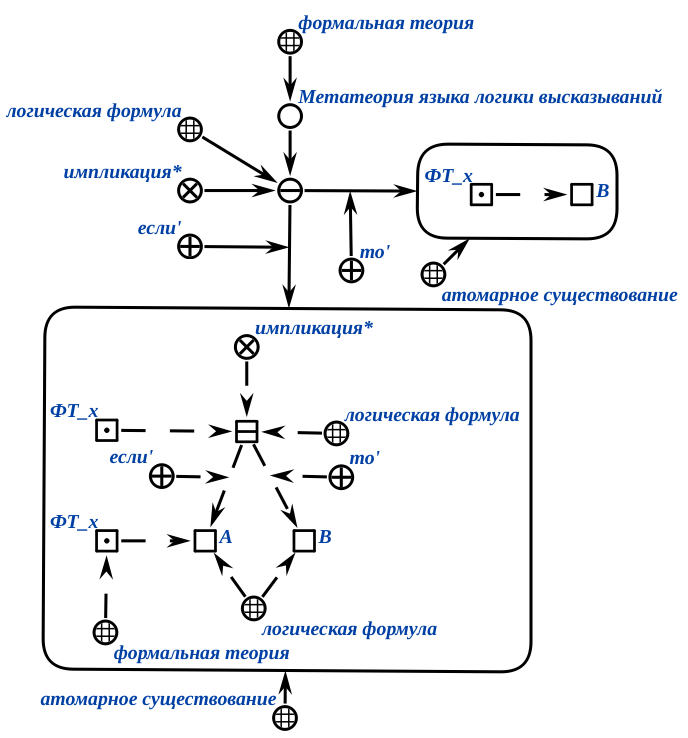
\includegraphics[width=0.9\linewidth, height=8cm]{figures/sc-agents/Modus_ponens.png}
%\end{figure}
%\end{frame}

\begin{frame}{\\Equivalent formula transformations}
\topline
\justifying
\vspace{10mm}

  This abstract sc-agent applies rules that put a logical formula into a particular form. It activates when an initiated action of the corresponding class appears in sc-memory. After checking the initiation condition, it converts the formula from one form to another without generating new domain knowledge. It returns formulas that are equivalent in meaning and differ in form, such as conjunctive or disjunctive normal form. The inference rule application agent often calls it when a formula can be converted into the form needed to apply a rule.
\end{frame}

\begin{frame}{}
\topline
\justifying
\vspace{10mm}

\begin{SCn}
\scnheader{Abstract sc-agent for equivalent formula transformations}
\begin{scnrelfromset}{abstract sc-agent decomposition}
	\scnitem{Abstract sc-agent for conversion to conjunctive normal form}
	\scnitem{Abstract sc-agent for conversion to disjunctive normal form}
	\scnitem{Abstract sc-agent for applying De Morgan's laws}
	\scnitem{Abstract sc-agent for equivalence transformations by definition}
	\scnitem{Abstract sc-agent for applying properties of negation}
	\scnitem{Abstract sc-agent for applying the idempotent law}
\end{scnrelfromset}
\end{SCn}
\end{frame}

\begin{frame}{}
\begin{SCn}
    \begin{scnrelfromset}{abstract sc-agent decomposition}
	\scnitem{Abstract sc-agent for applying the commutative law}
	\scnitem{Abstract sc-agent for applying the associative law}
	\scnitem{Abstract sc-agent for applying the absorption law}
	\scnitem{Abstract sc-agent for applying the law of non-contradiction}
	\scnitem{Abstract sc-agent for applying the double negation law}
	\scnitem{Abstract sc-agent for applying the splitting law}
\end{scnrelfromset}
\end{SCn}
\end{frame}

\begin{frame}{Abstract sc-agent for forward inference}
\topline
\justifying
	\setlength{\emergencystretch}{2em}
\vspace{10mm}

  This abstract sc-agent generates new knowledge from logical statements. An initiated action of the corresponding class activates it. Once its initiation condition has been checked, it repeatedly applies inference rules, generates knowledge in sc-memory, and checks a condition such as whether the target sc-structure's elements have appeared in memory. It takes a target structure, formulas used by the rule application agent, inference rules, and input and output structures. It produces an sc-structure representing a solution tree whose nodes are the applied rules that led to the required knowledge (the tree can be empty if inference failed to generate the required structure).
\end{frame}

%\begin{frame}{}
%\begin{figure}[H]
%	\caption{SCg-text. Specification of the forward inference agent}
%	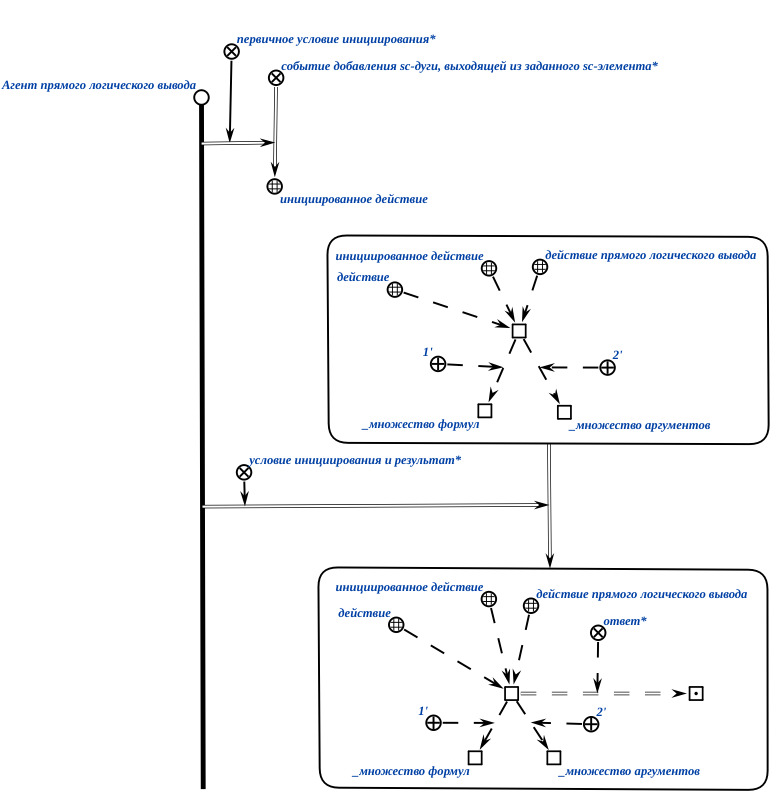
\includegraphics[width=0.9\linewidth, height=8cm]{figures/sc-agents/direct_inference_agent.png}
%\end{figure}
%\end{frame}

\begin{frame}{Backward inference agent}
\topline
\justifying
\vspace{10mm}

  This abstract sc-agent tests hypotheses. A refutation can reveal how to revise a premise and form a new hypothesis that may become a theorem. The agent activates when sc-memory contains an initiated backward inference action. Once its initiation condition has been checked, inference proceeds much like forward inference, except that rule search starts from conclusions rather than premises. The agent returns an inference tree that shows which rules can prove or refute the hypothesis.
\end{frame}

\begin{frame}{Synchronizing sc-agents}
\topline
\justifying
\vspace{10mm}

    A key feature of multi-agent problem solving is the ability to solve different problems in parallel, which requires their information processes to execute in parallel.
    An \textit{action in sc-memory} and a \textit{process in sc-memory} (an information process performed by an agent in semantic memory) are synonymous because sc-memory processes are deliberate and are carried out by \textit{sc-agents}. Literature on synchronization commonly uses the terms \textit{process} and \textit{process interaction}.
\end{frame}

\begin{frame}{\\Locks}
\topline
\justifying
\vspace{10mm}

To synchronize \textit{processes in sc-memory}, use a locking mechanism based on existing algorithms for synchronizing information processes in conventional systems. Lock-free algorithms are one possible direction for further development.

The \textbf{\textit{lock*}} relation links signs of \textit{actions in sc-memory} to signs of situational \textit{structures} whose elements are locked for all or part of the action's execution. Each such \textit{structure} belongs to a \textit{lock type}.

The first component of a tuple of the \textbf{\textit{lock*}} relation is the sign of the \textit{action in sc-memory}, and the second is the sign of the locked \textit{structure}.
\end{frame}

\begin{frame}{\\Processes in sc-memory}
\topline
\justifying
\vspace{10mm}


\begin{SCn}
\scnheader{process in sc-memory}
\scnrelfrom{partition}{classification of sc-memory processes by execution synchronization}
\begin{scnindent}
\begin{scneqtoset}
	\scnitem{action to search for sc-elements}
	\scnitem{action to generate sc-elements}
	\scnitem{action to delete sc-elements}
	\scnitem{action to place a lock of a given type on an sc-element}
	\scnitem{action to remove a lock from an sc-element}
\end{scneqtoset}
\end{scnindent}
\end{SCn}
\end{frame}

\begin{frame}{}
	\topline
	\justifying
	\vspace{10mm}

Sometimes synchronization requires grouping several elementary sc-memory actions into a single indivisible action. No other process can read or modify the participating sc-elements before the action completes. A process requesting access waits until then and can subsequently operate on the elements according to the synchronization rules.

An \textit{action to search for sc-elements} places every element found and retained by a process under that process's \textit{modification lock}. This preserves the integrity of the knowledge base fragment the process is using. Searching and automatically placing the lock must be one \textit{sc-memory transaction}.

\end{frame}

\begin{frame}{}
	\topline
	\justifying
	\setlength{\emergencystretch}{2em}
	\vspace{10mm}

This approach also prevents a process from generating or deleting an \textit{sc-connector} incident to an \textit{sc-element} that another process has locked against modification. The second process must first find the \textit{sc-element} and try to place its own modification lock, creating a lock conflict (\textit{deadlock*}).

Any sc-element generated by a process is automatically placed under that process's full lock. Generation and automatic locking must be a single \textit{sc-memory transaction}. If necessary, the generated elements can be deleted without their temporary existence affecting other processes. They can also be unlocked if the information generated may be useful later.
\end{frame}

\begin{frame}{}
	\topline
	\justifying
	\vspace{10mm}

A process requesting a lock of any type on an sc-element locked by another process cannot acquire it until the other process releases the element. To detect and resolve \textit{deadlocks}, the waiting request must be represented explicitly. The proposed \textit{planned lock*} relation records which processes are trying to lock an already locked \textit{sc-element} and is analogous to the \textit{lock*}.
\end{frame}

\begin{frame}{}
	\topline
	\justifying
	\setlength{\emergencystretch}{2em}
	\vspace{10mm}

This mechanism also regulates search because finding and retaining an sc-element requires a \textit{modification lock}. A process can apply a \textit{modification lock} after another process has placed a \textit{deletion lock} on the same element. The \textit{planned lock*} relation is unnecessary in that case.

Checking whether an sc-element has a lock and then placing either a lock or a planned lock, with a priority if needed, must be a single transaction.
\end{frame}

\begin{frame}{Relationship to SCP}
\topline
\justifying
\vspace{10mm}


    The basic programming language of OSTIS systems distinguishes methods and skills that can be fully represented in the knowledge base from lower-level skills that interpret them. This gives OSTIS systems \uline{platform independence}, whether the implementation uses a software \textit{OSTIS platform} or an \textit{associative semantic computer}.
    \par \textit{SCP} is the proposed basic language for programs that process \textit{SC-code} texts. \textbf{\textit{SCP}} is a graph-based procedural programming language for efficient processing of \textit{sc-texts}. It supports parallel asynchronous programming.
\end{frame}

\begin{frame}{}
\topline
\justifying
\vspace{10mm}

SCP programs use SC-code and any of its external representations for data. SCP itself is based on SC-code, so scp-programs can process other programs and even themselves as data. This enables reconfigurable programs. To reconfigure a program during interpretation, the SCP interpreter (the Abstract scp-machine) must give each executable copy of the original program its own identity. Such a copy, generated from an scp-program, is called an scp-process. If the sign of an action in sc-memory belongs to the set of scp-processes, its decomposition contains only signs of elementary actions (scp-operators) that an implementation of the Abstract scp-machine can interpret (the interpreter for scp-programs).
\end{frame}

\begin{frame}{The basic model for processing sc-texts}
\topline
\justifying
\vspace{10mm}

\begin{textitemize}
    \item \textit{SCP} programs are written using the same unified semantic networks as the information they process. At the basic level, \textit{SCP syntax} therefore coincides with \textit{SC-code syntax}.
    \item Interpreting \textit{scp-programs} involves creating a unique \textit{scp-process}.
    \item Several independent \textit{sc-agents} can run in shared memory simultaneously. The distributed \textit{OSTIS platform} allows separate copies of agents to run on different servers. \textit{SCP} also allows asynchronous parallel subroutine calls followed by synchronization, and can execute operators in parallel within one \textit{scp-program}.
    \end{textitemize}
\end{frame}

\begin{frame}{}
\topline
\justifying
\vspace{10mm}
\small

\begin{textitemize}
    \item Moving an \textit{sc-agent} between systems requires transferring a \textit{knowledge base} fragment, without operations specific to the \textit{OSTIS platform}.
	\item Using the same language for \textit{sc-agent} specifications, their programs, and the knowledge they process reduces the number of specialized tools for designing knowledge processing machines. More general components simplify their development.
	\item A unique \textit{\mbox{scp-process}} is created to interpret each \textit{scp-program}. This allows the execution plan to be optimized before or even during execution without changing the program's general algorithm. It also makes self-reconfiguring programs possible.
\end{textitemize}
\end{frame}

\begin{frame}{}
\topline
\justifying
\vspace{10mm}

Each \textbf{\textit{scp-program}} is a generalized \textit{sc-structure} describing one possible decomposition of actions of a given class that run in sc-memory. The sign of the \textit{sc-variable} corresponding to the specific decomposed action is a \textit{key sc-element\scnrolesign} of the \textbf{\textit{scp-program}}. The program explicitly marks that sign as a member of \textit{scp-processes}.

An action belonging to \textit{scp-processes} is guaranteed to decompose only into signs of elementary actions (\textit{scp-operators}) interpretable by an implementation of the \textit{Abstract scp-machine}.
\end{frame}

\begin{frame}{}
\topline
\justifying
\vspace{10mm}

Each \textbf{\textit{scp-program}} therefore describes the generalized decomposition of an \textit{\mbox{scp-process}} into interrelated \textit{scp-operators} and specifies any arguments of that \textit{scp-process}.

Each \textbf{\textit{scp-program}} describes a sequence of elementary operations on a semantic network needed to perform a more complex action of a given class.
This example illustrates a simple \textit{scp-program} with three \textit{scp-operators}. The program checks whether a given set (the first parameter) contains the given element (the second parameter) and adds the element if it is absent.
\end{frame}

%\begin{frame}{}
%\begin{figure}[H]
%    \caption{SCg-text. Example of an scp-program}
%	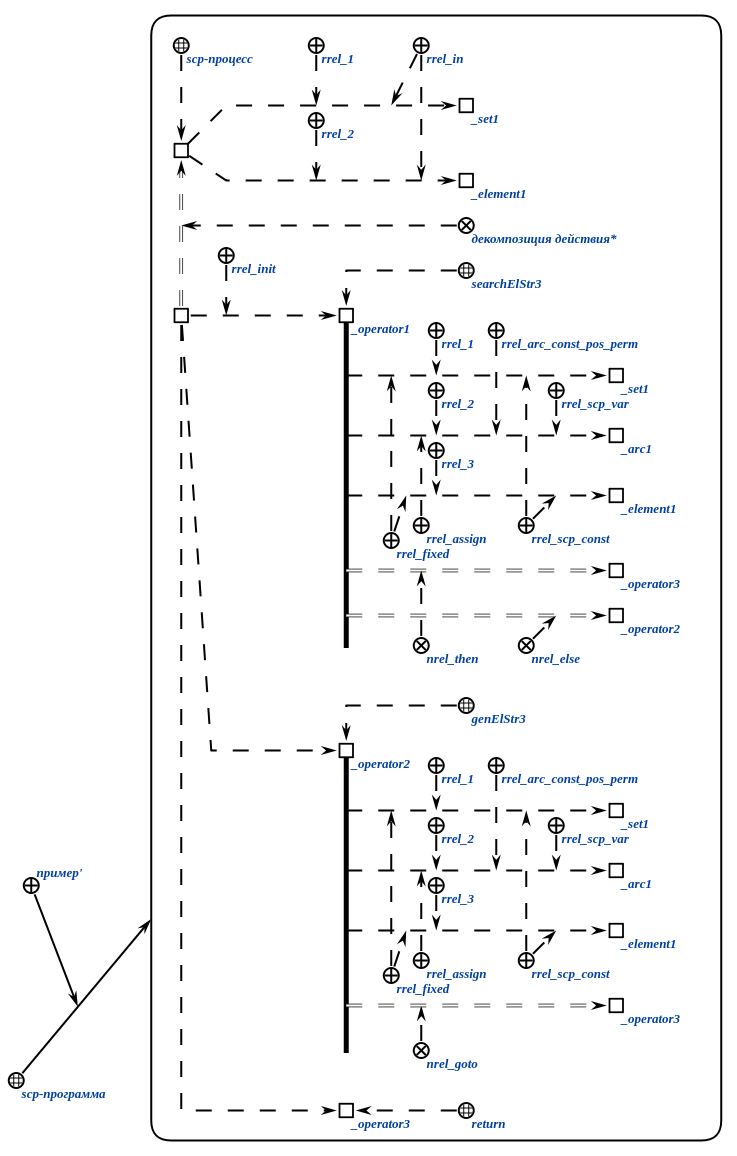
\includegraphics[width=0.9\linewidth, height=8cm]{figures/sc-agents/program_example.png}
%\end{figure}
%\end{frame}

\begin{frame}{}
\topline
\justifying
\vspace{10mm}

\textbf{\textit{Agent scp-programs}} are a particular type of \textit{scp-program} and deserve separate attention because they are used most often. They implement knowledge processing agents and have a fixed set of exactly two \textit{input parameters\scnrolesign}. The first parameter is the sign of a binary ordered pair. That pair is the second component of a \textit{primary initiation condition*} tuple for the abstract \textit{sc-agent} whose set of \textit{sc-agent programs*} includes the \textbf{\textit{agent scp-program}}. In effect, the pair describes the class of events that the agent responds to.

The second parameter is the \textit{sc-element} directly associated with the event that initiated the \textit{sc-agent}, such as the generated or deleted \textit{sc-arc} or \textit{sc-edge}.
\end{frame}

\begin{frame}{Implementing abstract sc-agents in SCP}
\topline
\topline
\justifying
\vspace{10mm}

    \begin{textitemize}
    \item common principles for interaction between \textit{sc-agents} and \textit{OSTIS system} users through shared \textit{sc-memory};
\item when a construct appears in sc-memory that satisfies the initiation condition of an \textit{abstract sc-agent} implemented in \textit{SCP}, an \textit{scp-process} is generated and initiated in \textit{sc-memory}. Its template is the \textit{agent scp-program} specified in the set of programs for the corresponding \textit{abstract sc-agent};
\item each \textit{scp-process} corresponding to an \textit{agent scp-program} can be associated with structures that describe locks of different types. Concurrent \textit{scp-processes} are synchronized in the same way as other \textit{actions in sc-memory};
\end{textitemize}
\end{frame}

\begin{frame}{}
\topline
\justifying
	\setlength{\emergencystretch}{2em}
\vspace{10mm}


\begin{textitemize}
    \item an \textit{scp-process} can create child \textit{scp-processes}. Additional internal locks synchronize them if needed. From the viewpoint of \textit{processes in sc-memory}, each \textit{scp-process} is therefore an atomic and complete act of an \textit{sc-agent};
    \item to prevent unwanted changes to the body of an \textit{scp-process}, the whole construct generated from the \textit{scp-program} (the entire process text) must be covered by the \textit{full lock} associated with the \textit{scp-process};
\end{textitemize}
\end{frame}

\begin{frame}{}
\topline
\justifying
	\setlength{\emergencystretch}{2em}
\vspace{10mm}

\begin{textitemize}
\item all constructs generated during an \textit{scp-process} are automatically covered by its \textit{full lock}. The sign of the lock structure itself and all its metadata are also included in that structure;
\item when necessary, a construct can be manually unlocked or locked with any lock type using the corresponding \textit{scp-operators} of the class \textit{lock management scp-operator};
\item once an \textit{scp-process} completes, its text is generally removed from \textit{\mbox{sc-memory}} and all locked constructs are released (the signs of structures denoting locks are destroyed);
\end{textitemize}
\end{frame}

\begin{frame}{}
\topline
\justifying
\vspace{10mm}

\begin{textitemize}
\item each \textit{scp-operator} is an atomic \textit{action in sc-memory}. To avoid excessive system constructs, operators share the locks for the whole \textit{scp-process} instead of introducing per-operator locks. The agents of the \textit{Abstract scp-machine} therefore interpret \textit{scp-operators} using only the locks for the entire \textit{scp-process};
\item normally, a particular \textit{class of actions} for an individual \textit{scp-program} is not introduced explicitly. The broader \textit{scp-process} class is used unless some other requirement calls for a separate \textit{class of actions}.
\end{textitemize}
\end{frame}
